\chapter{Fundamentação Teórica}

Este capítulo aborda em detalhes os principais conceitos e tecnologias que fundamentam o projeto, incluindo temas como Internet das Coisas (\textit{IoT}), Sistemas Distribuídos, 
redes de comunicação como Wi-Fi e Bluetooth, protocolo de comunicação HTTP, desenvolvimento de software para a plataforma Android, características do microcontrolador ESP32, monitoramento de 
exposição ao monóxido de carbono e trabalhos relacionados. Todos os tópicos citados possuem papel crucial no desenvolvimento da solução proposta no trabalho de conclusão de curso. Dessa forma, o
objetivo é fornecer ao leitor uma visão abrangente das competências técnicas e teóricas aplicadas em sua execução.

\section{Internet das Coisas}

O termo \textit{Internet das Coisas} (\textit{IoT}, da expressão em inglês \textit{Internet of Things}) foi utilizado primeiramente em 1999 pelo então pesquisador do \textit{Massachusetts Institute of Technology} (MIT) Kevin Asthon em 
uma apresentação na Procter \& Gamble (P\&G) sobre a tecnologia do \textit{Radio Frequency Identification} (RFID). O RFID é uma tecnologia utilizada para a identificação e rastreamento de objetos, animais ou pessoas 
via ondas de rádio. Portanto, Asthon pontuou a possibilidade de utilizar tal ferramenta para gerenciar a cadeia de suprimentos da empresa, pois sua capacidade de ler vários emissores simultaneamente, sem a necessidade de linha de visão direta entre o leitor 
e a tag (ao contrário do códigos de barras) torna o monitoramento de cada produto nos distintos pontos de transporte mais preciso. A ideia do autor consiste na responsabilidade dos próprios objetos sobre a coleta de dados
e reação aos estímulos do ambiente, pois os computadores podem reduzir custos e o desperdício apenas tomando decisões com base na sua própria observação do mundo externo \cite{iot-first-definition}.

\textit{IoT} possui muitas definições. Embora não haja um consenso para uma definição única, podemos discutir sobre seu impacto na sociedade atual e aspectos importantes que toda solução na área possui. No livro \textit{The Internet  of Things}, escrito por 
Samuel Greengard, o tema é abordado como um evento disruptivo, onde a linha que separa o humano e a tecnologia se torna cada vez menos visível, porém o texto aborda não somente a capacidade de conexão entre as máquinas, e sim a autonomia 
e ``inteligência'' crescente dos sistemas embarcados \cite[pp. 17]{book-iot}. Essa visão de tecnologia integrada no cotidiano é o conceito que o autor Mark Weiser aborda no seu artigo denominadao \textit{The Computer for the 21st Century}. A computação ubíqua 
é o processo de tornar os computadores ``invisíveis'' aos nossos olhos, desenvolvendo a comunicação com tais ferramentas o mais próximo possível da forma humana, ou seja, o dispositivo tem conexão com a rede e responde aos estímulos do usuário por 
interfaces naturais, por exemplo, a fala e gestos com as mãos \cite{ubiquitous-computing}.

Portanto, o significado mais comum de \textit{IoT} talvez seja a de dispositivos eletrônicos conectados na internet, permitindo 
enviar e receber dados do ambiente real. No entanto, apenas conectar dispositivos não é uma solução em Internet das Coisas, pois essa 
área envolve o uso de protocolos de comunicação, eletrônica de baixo consumo energético, plataformas em nuvens e outras inúmeras 
áreas do conhecimento. Os dados coletados de sensores atuam como combustível para a execução de um fluxo de tomada de decisão \cite{iot-cycle}. 

\begin{figure}[ht]
    \centering
    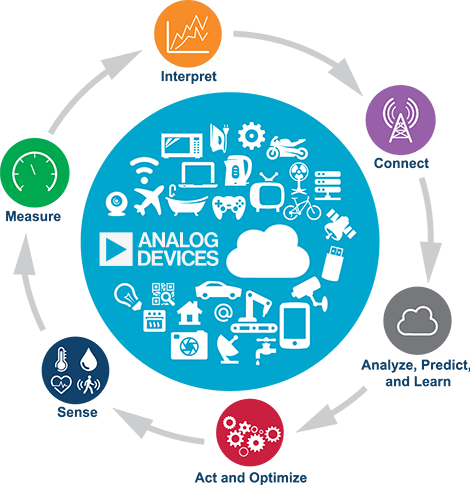
\includegraphics[width=.45\textwidth]{img/iot-cycle.png}
    \caption{Ciclo de IoT. Fonte:\cite{iot-cycle}}\label{figIoTCycle}
\end{figure}

Atualmente, a coleta de dados e o uso de ferramentas de análise são os principais recursos de empresas competitivas no gerenciamento de suas atividades. Com o 
avanço da área de telecomunicações, as organizações têm potencial de transformar grandes volumes de dados em \textit{insights} poderosos, que orientam a tomada de 
decisões da equipe de gestão, em busca de eficiência. Portanto, a Internet das Coisas representa uma tendência forte e disruptiva na sociedade.

\section{Sistemas Distribuídos}

``Um sistema distribuído é aquele no qual os componentes localizados em computadores interligados em rede se comunicam e coordenam suas ações apenas passando mensagens.'' \cite[pp. 1]{sistemas-distribuidos-coulouris2013}.
A definição apresentada pelo autor leva em conta dois importantes fatores: o primeiro é representado pela comunicação via rede de computadores, e o segundo está relacionado ao provisionamento de um serviço.
O mundo atual oferece inúmeros exemplos da importância dos sistemas distribuídos no desenvolvimento socioeconômico: a modalidade de educação à distância \cite{mec-ead}, no qual serviços web e compartilhamento
multimídia são responsáveis por possibilitar o acesso ao ensino de qualidade ao público distante fisicamente dos grandes centros de ensinos, como, por exemplo, cidades do interior ou comunidades ribeirinhas; o comércio digital, onde a arquitetura do sistema deve suportar picos de acesso em determinados períodos do ano e controle
de concorrência na compra de produtos, deve-se ao crescimento do seguimento de \textit{e-Commerce},
resultou em um faturamento superior à R\$ 180 bilhões de reais em 2023 no Brasil, de acordo com dados da Associação Brasileira de Comércio Eletrônico \cite{abcomm-ecomerce}; e redes \textit{blockchain}, pois as transações distribuídas devem ser auditáveis e transparentes, além do funcionamento descentralizado \cite{juliana-blockchain}, exemplo 
das criptomoedas, pois a tecnologia permite a transferência de recursos e o armazenamento de todas as operações.  

Portanto, o sistema distribuído tem foco no compartilhamento de recursos. Na web, a implementação de arquitetura mais comum é o modelo cliente-servidor, pois
um número grande de aplicações utiliza essa premissa, por exemplo, plataformas de redes sociais, jogos online e serviços bancários.
Ao nível do Sistema Operacional, a comunicação entre processos executados em diferentes computadores interligados em rede é essencial para o gerenciamento e acesso aos recursos distribuídos.
Nesse contexto, um cliente, que pode ser um processo ou aplicativo, realiza uma solicitação ao servidor para acessar ou manipular um recurso, como arquivos, impressoras, ou mesmo capacidade de processamento. O servidor, 
ao receber essa solicitação, desencadeia uma série de operações internas, que podem incluir desde a autenticação do cliente até a busca de dados em um banco de dados distribuído. Em seguida, o servidor 
retorna o resultado ao cliente em espera, completando o ciclo de comunicação do tipo requisição e resposta \cite[pp. 16]{sistemas-distribuidos-coulouris2013}.

\section{HTTP: Fundamentos e Impacto na Web}

O HTTP (do inglês \textit{HyperText Transfer Protocol}) é o protocolo pertencente à camada de aplicação
responsável por definir a estrutura de mensagens HTTP e a forma do programa cliente e do programa servidor 
trocarem suas mensagens individuais. Seu funcionamento obedece à arquitetura cliente-servidor, ou seja, o
usuário (geralmente um navegador Web) envia uma requisição ao servidor, que deverá processá-la e responder 
com um resultado, denominado resposta. O exemplo descrito é o uso de navegadores para requisitar uma página web, porém 
o protocolo HTTP é extensível, pois a comunicação descrita se aplica ao acesso dos mais variados tipos de recursos, graças a
um conceito denominado URL (Uniform Resource Locator), responsável por identificar de maneira única um objeto na internet \cite[pp. 72]{redes-kurose2010}.

\subsection{Padrão de mensagem HTTP}

No protocolo, existem dois tipos de mensagem: requisição e resposta. Na mensagem de requisição, temos o elemento
chamado \textbf{método}, esse campo define qual a ação que o usuário deseja executar, sendo comum o uso de verbos
como GET, POST, HEAD, PUT e DELETE. Por exemplo, ao realizar o preeenchimento de um formulário de cadastro do site, o
navegador web realiza uma requisição do tipo POST ao servidor, pois sua intenção é a criação de um recurso,
neste caso, a nova conta. A ação é executada sobre um \textbf{caminho}, que corresponde à organização interna dos recursos 
dentro do servidor, por exemplo, as informações sobre produtos estão no caminho ``/product''. O \textbf{cabeçalho} contém informações como: preferência de linguagem,
credenciais de acesso, tipo de conteúdo na mensagem, entre outros. Por fim, o último campo é o \textbf{corpo da mensagem}, 
onde ficam armazenados os dados \cite[pp. 77]{redes-kurose2010}.

\begin{figure}[ht]
    \centering
    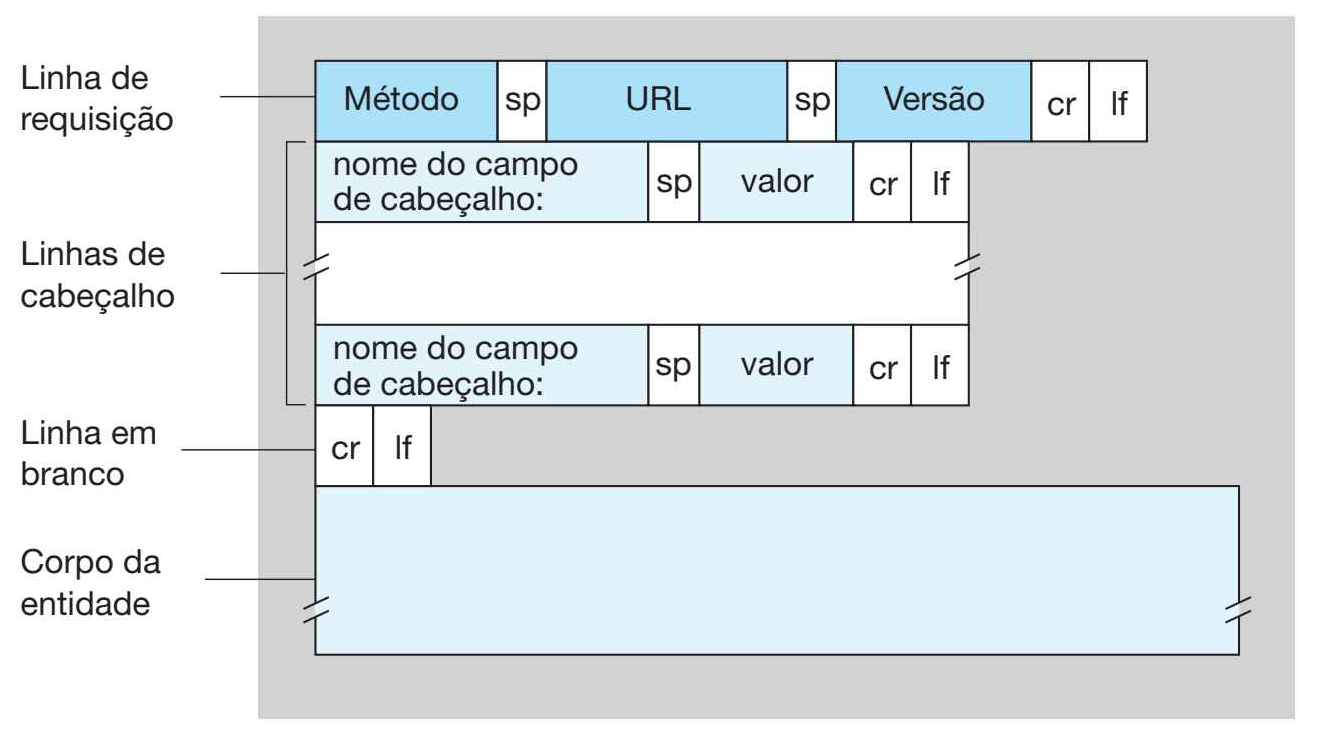
\includegraphics[width=.55\textwidth]{img/mensagem-http-solicitação.png}
    \caption{Padrão de mensagem de solicitação HTTP. Fonte:\cite{redes-kurose2010}}\label{figMessageRequest}
\end{figure}

A mensagem de resposta é constituída de 3 componentes principais: linha de estado, linha de cabeçalho e corpo de entidade. Na \textbf{linha de estado}, um campo
interessante é o \textit{status code}, número pré-definido que indica se o resultado da requisição foi bem-sucedido, ou não, assim como o motivo. No \textbf{cabeçalho}
são adicionadas pelo servidor informações como o tipo do objeto e seu tamanho em bytes. Por último, o \textbf{corpo da mensagem} em si, contendo os dados solicitados \cite[pp. 78]{redes-kurose2010}.

\begin{figure}[ht]
    \centering
    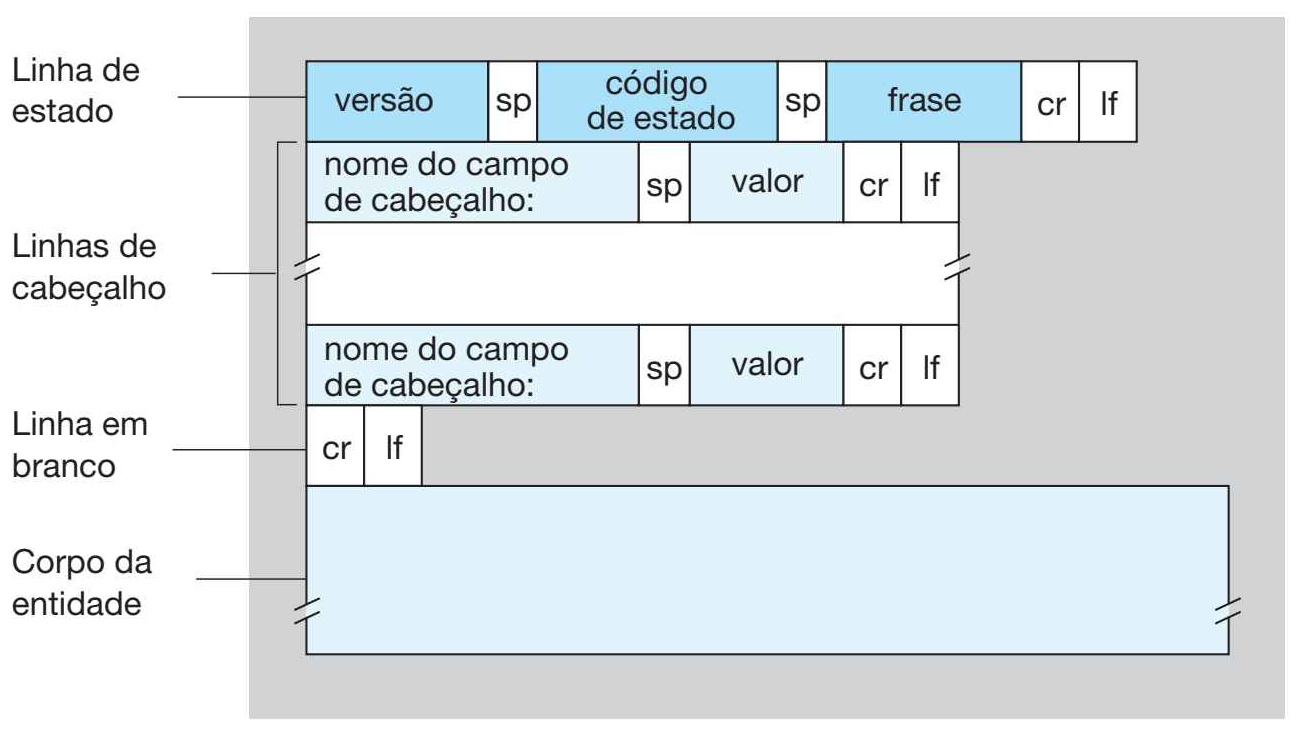
\includegraphics[width=.55\textwidth]{img/mensagem-http-resposta.png}
    \caption{Padrão de mensagem de resposta HTTP. Fonte:\cite{redes-kurose2010}}\label{figMessageResponse}
\end{figure}

\subsection{API}

API é o acrônimo de \textit{Application programming interface}, cuja função é estabelecer um conjunto de padrões e funções
para que diferentes sistemas de software possam se comunicar, executar ações e trocar dados \cite{api-definition}. Por exemplo, a biblioteca
\textit{OpenGL} foi construída como uma API de computação gráfica, responsável por renderizar e modelar objetos no espaço tridimensional independente
de dispositivos de \textit{hardware} \cite{opengl-example}. Outra API bastante utilizada é a \textit{Google Maps API}, pois é um serviço da empresa Google\textsuperscript{\textregistered} 
para acessar dados de geolocalização muito utilizado em sites de hotéis, divulgação de lojas e uso pessoal para encontrar lugares \cite{google-maps-example}. Portanto, API é um recurso 
prático, pois é transparente ao desenvolvedor de software, porém, sem a necessidade de conhecer os procedimentos internos.

O padrão REST (Representational State Transfer) é um estilo de arquitetura de sistemas web 
que provê acesso uniforme aos recursos de um servidor, por meio de uma interface coerente que aplica uma mudança de
estado através das operações básicas do protocolo HTTP, com importância maior aos dados do que a operação e baixo acoplamento entre sistemas. 
Além disso, essa interface de comunicação de sistemas via HTTP garante que cada recurso seja acessível por
uma URL e a interação da API, seja \textit{stateless}, ou seja, a requisição contém toda a informação necessária
para sua execução pelo servidor \cite[pp. 384--386]{sistemas-distribuidos-coulouris2013}. 

Portanto, o desenvolvimento de uma API no padrão REST é útil para a integração entre diferentes sistemas e  padronização das mensagens 
utilizando o protocolo HTTP. As principais vantagens na escolha do REST são: interoperabilidade, onde o 
dispositivo eletrônico envia os dados obtidos e o aplicativo Android consome os eventos, realizando a 
gestão da conta do usuário, com todas essas operações na API comunicadas de maneira uniforme; independência 
de estado, já que o dispositivo pode perder a conexão, mas ao restabelecê-la, deve garantir a comunicação correta; e simplicidade 
na evolução do sistema, uma vez que o modelo suporta comunicação com múltiplos clientes.

\begin{figure}[ht]
    \centering
    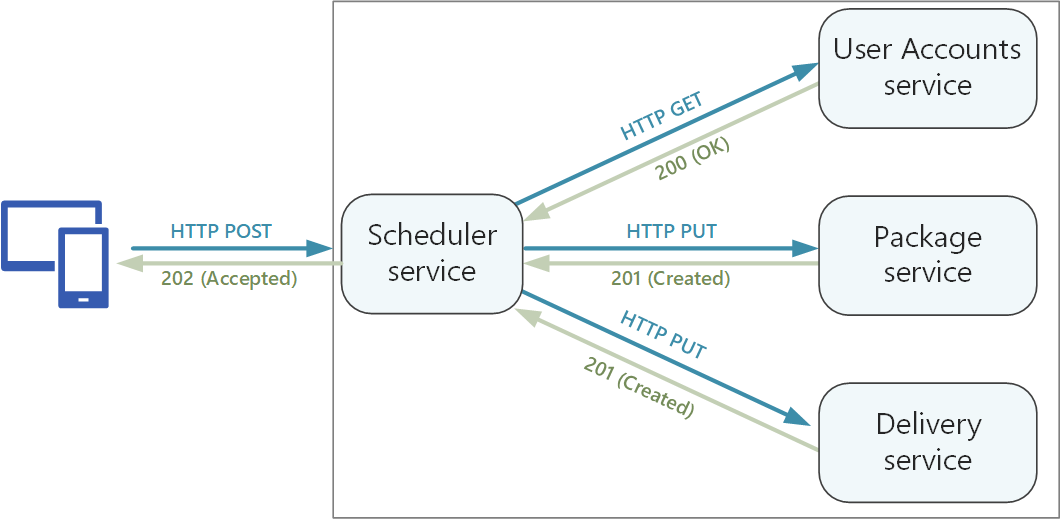
\includegraphics[width=.45\textwidth]{img/api-design.png}
    \caption{Example de design de API para microsserviços. Fonte:\cite{example-design-api}}\label{figAPIDesign}
\end{figure}

\section{Desenvolvimento de aplicativos Android}

O Android possui uma extensa documentação, fornecendo os fundamentos para o desenvolvimento de 
aplicativos de alta qualidade e resilientes. Portanto, essa seção abordará as melhores práticas e recomendações
de arquitetura para a construção de aplicativos com uma experiência de usuário fluida e consistente. Tais práticas envolvem o profundo
conhecimento de componentes de aplicativo, fluxos de trabalho e ciclo de vida da camada de visualização. Ao seguir uma arquitetura, 
o desenvolvedor de \textit{software} consegue melhorar sua produtividade e a qualidade de entregas, pois uma base de código aderente ao 
padrão escolhido facilita a manutenção, desenvolvimento de novas funcionalidades e promove a colaboração entre equipes \cite{google-developers-guideline}.

\subsection{Recomendação de Arquitetura}

Um princípio muito usado na área de desenvolvimento de software é o chamado \textit{separation of concerns}, ou separação de responsabilidades. Esse conceito, no ecossistema Android,
atua na divisão do sistema em partes menores, específicas para uma determinada função e com um objetivo bem definido. Por exemplo, não misturar lógica de 
negócio ou acesso aos dados na camada de visualização (UI), tornando-a  responsável apenas pela interação com o usuário. Diante disso, a documentação recomenda a separação em (pelo menos)
duas camadas principais: \textit{UI} e \textit{Data}. A camada de \textit{UI} é responsável por exibir os dados do aplicativo, refletindo a mudança na tela em resposta às
interações do usuário (como cliques ou pressionamento de botões) ou a eventos externos (como a resposta de uma requisição de rede). Por sua vez, a camada \textit{Data} fornece à camada de \textit{UI} 
um acesso simplificado aos dados, além de abrigar a lógica de negócio e o gerenciamento adequado de cada tipo de dado. Opcionamente, pode-se adicionar uma terceira camada entre as duas chamada de \textit{Domain Layer}.
Sua função é intermediar a comunicação entre as duas camadas, abstraindo chamadas e eventos em um lugar centralizado \cite{google-developers-guideline}.

\begin{figure}[ht]
    \centering
    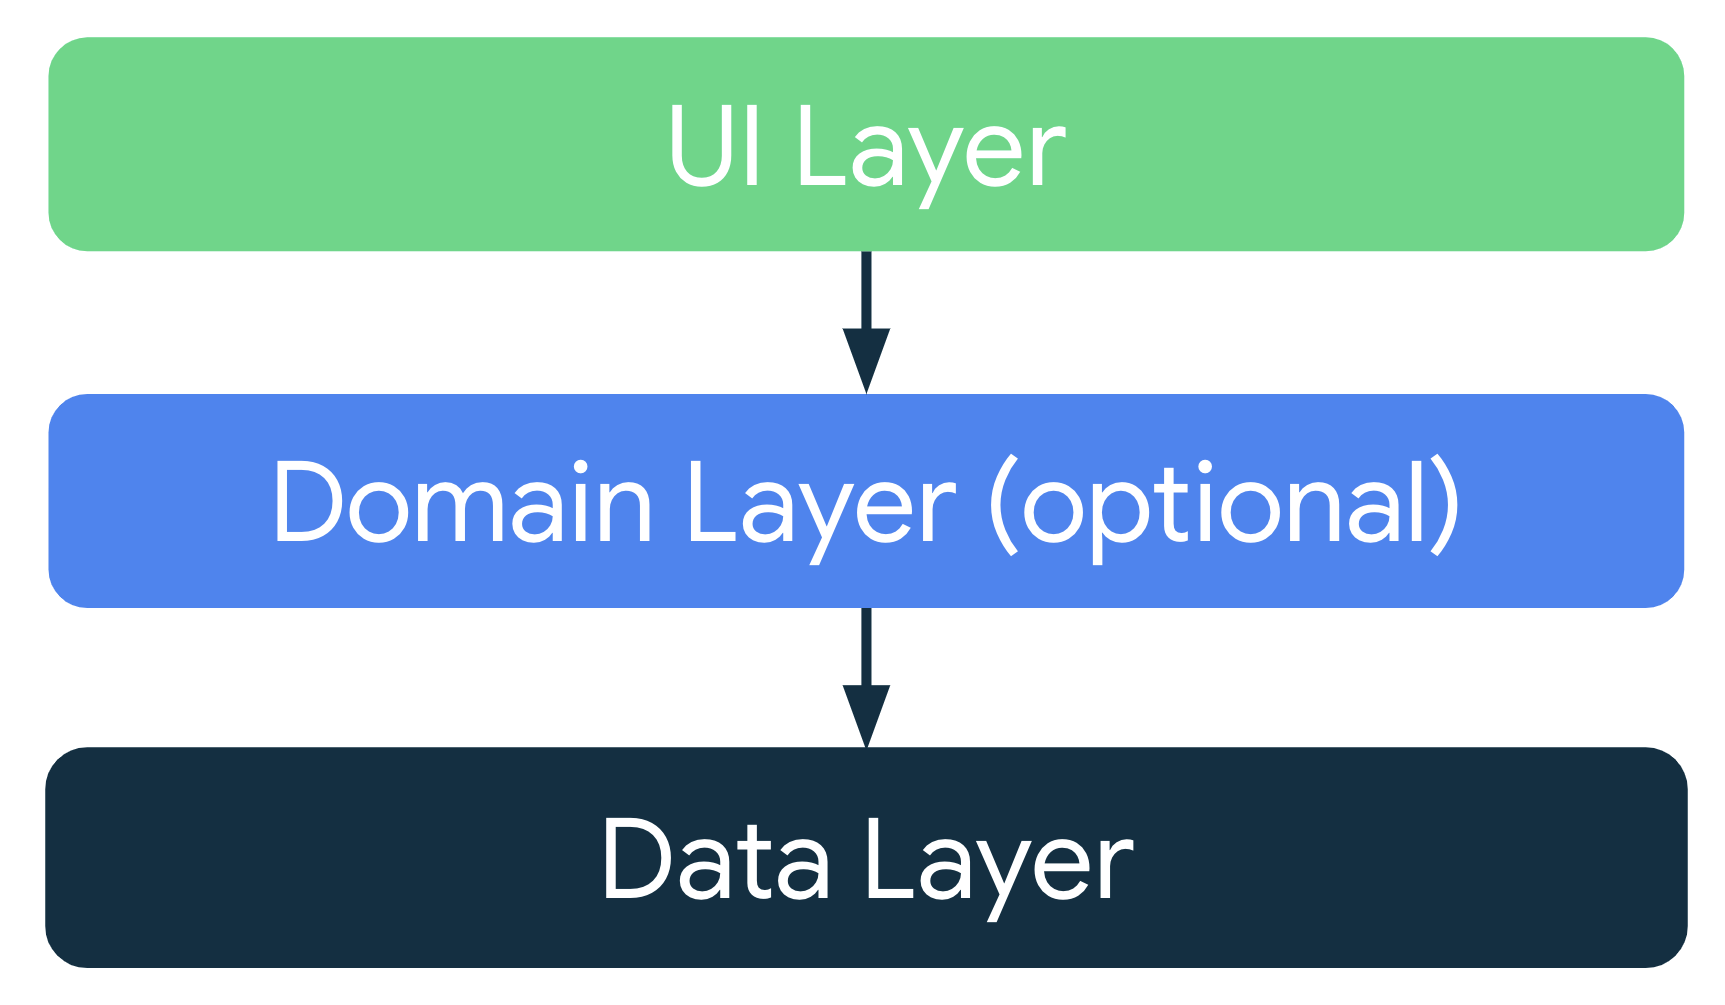
\includegraphics[width=.73\textwidth]{img/app-android-layers.png}
    \caption{Camadas de arquitetura (App). Fonte:\cite{google-developers-guideline}}\label{figAppLayer}
\end{figure}

\subsection{Ciclo de vida da atividade}\label{ciclo-de-vida}

O \textit{Activity lifecycle} (ciclo de vida de uma atividade) descreve todos os estados pelos quais uma activity passa, do momento em que é criada
até quando é destruída. Uma \textit{activity} é uma classe que fornece uma janela para o aplicativo desenhar sua interface de usuário, pois um projeto Android 
inicia sempre com uma \textit{activity}. O ciclo de vida de uma \textit{activity} passa por cinco etapas: 
\textit{initialized}, \textit{created}, \textit{started}, \textit{resumed}, \textit{destroyed}. A seguir, será explicado o que ocorre em cada 
uma delas e suas especificidades.

\begin{figure}[ht]
    \centering
    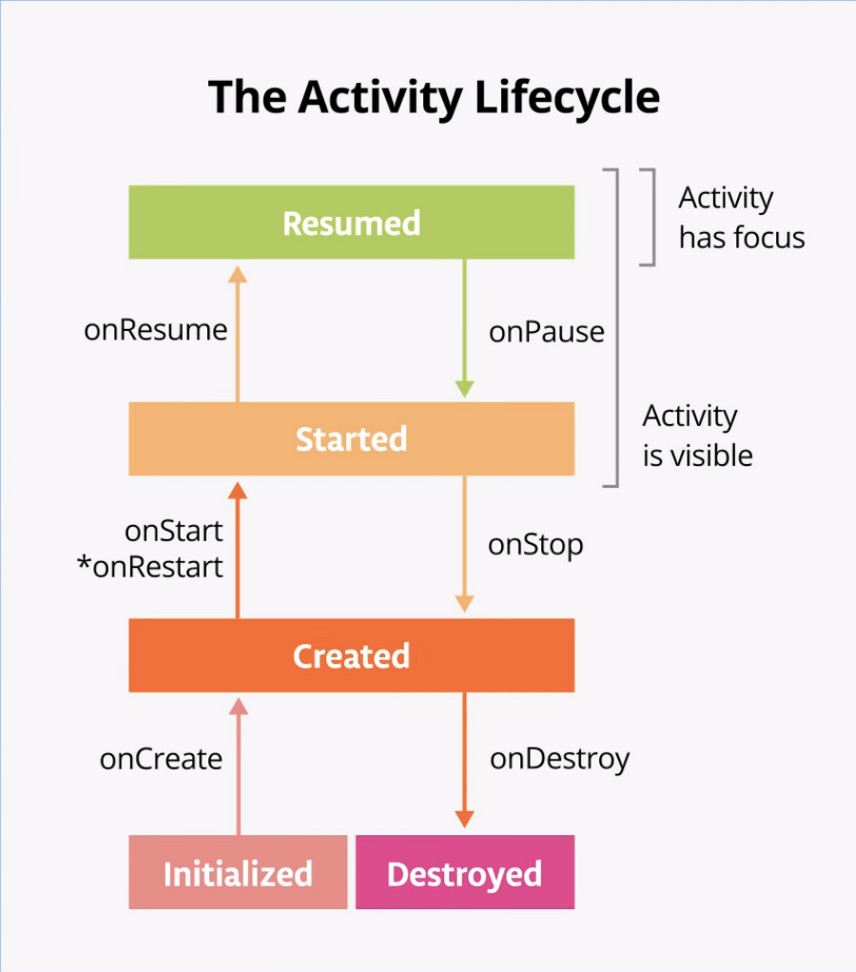
\includegraphics[width=.37\textwidth]{img/activity-lifecycle.png}
    \caption{Ciclo de vida de uma \textit{activity}. Fonte:\cite{google-developers-activity-lifecycle}}\label{figActivityLifeCycle}
\end{figure}

Quando a \textit{activity} é criada pelo sistema, o estado \textit{created} é ativado. Nesse estágio, os recursos da interface gráfica 
são inicializados, porém, a janela ainda não está disponível ao usuário. A partir do estado \textit{started}, os componentes da \textit{activity} são exibidos e a tela se torna visível, porém sem interação.
O estado \textit{resumed} é o aplicativo em primeiro plano, recebendo interações com o usuário em pleno exercício de suas funções. No entanto, se o usuário realizar uma ação que tire 
o foco do aplicativo (como verificar um e-mail após receber uma notificação), a \textit{activity} entrará no estado de pausa (paused).
Caso o usuário volte ao aplicativo, a \textit{activity} retoma os estados \textit{started} e \textit{resumed}, restaurando a interação. No entanto, se o usuário não retornar e a \textit{activity} for fechada, 
ela passará para o estado \textit{destroyed}, encerrando seu ciclo de vida \cite{google-developers-activity-lifecycle}.

\subsection{Arquitetura MVVM}

O Model-View-ViewModel (MVVM) é um padrão de projeto de software criado por engenheiros da Microsoft\textsuperscript{\textregistered} 
cuja função é separar a lógica de software da configuração de interface do usuário. Além disso, esse padrão de projeto facilita a aplicação de testes de unidades e reutilização 
de código. O \textit{Model} é o componente não visual que armazena a lógica de negócio e o modelo de dados do domínio da aplicação, pois recebe e envia dados da \textit{ViewModel} 
para que ela interaja com a \textit{View}. A \textit{View} são os elementos visíveis de interação com o usuário, pois recebem entradas de dados e eventos de \textit{UI}. Por fim, a
\textit{ViewModel} implementa propriedades e funções para que a \textit{View} se associe aos dados e receba eventos de notificação para renderizar atualizações na camada de \textit{Model} \cite{mvvm-documentation}.

\begin{figure}[ht]
    \centering
    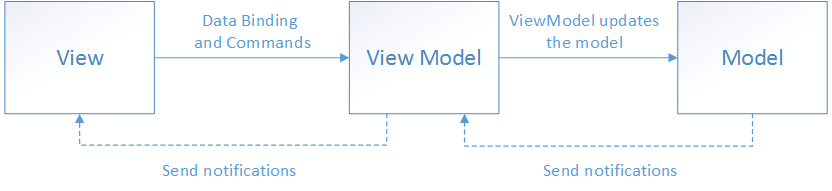
\includegraphics[width=.57\textwidth]{img/mvvm-pattern.png}
    \caption{MVVM. Fonte:\cite{mvvm-documentation}}\label{figMVVM}
\end{figure}

No Android, a \textit{ViewModel} possui o papel de persistência de dados quando ocorre mudança 
de estado na tela. Essas mudanças de estado são dinâmicas, como a rotação de tela ou troca de aplicativo após notificação, e, por isso, 
podem resultar em perda de dados armazenados em variáveis ou componentes visuais. A classe \textit{ViewModel}, fornecida pelo próprio 
\textit{Framework} Android, é desenvolvida para manter os dados resilientes às mudanças da interface gráfica, garantindo que informações significativas, como entradas de 
formulário e respostas de um \textit{backend}, permaneçam preservados durante a recriação da tela e componentes. Todo \textit{ViewModel} é gerenciado por um objeto 
que implementa a interface \textit{ViewModelStoreOwner}, pois seu estado é preservado durante os estados de \textit{paused}, \textit{stoped} e \textit{started} do seu \textit{Owner}, sendo destruído
juntamente com a tela, porém fechando todas suas operações com segurança. Portanto, ele funciona como um intermediário entre os dados (\textit{model}) e
os elementos visuais (\textit{view}), aderente às especificidades do ciclo de vida de uma aplicação android \cite{google-developers-viewmodel}.

\section{ESP32}

ESP32 é uma família de microcontroladores desenvolvida pela empresa Espressif Systems rica em recursos como conectividade Wi-Fi e Bluetooth projetado para aplicações de IoT. 
Está presente em soluções de automação, por apresentar vantagens como: design robusto, ao poder operar entre diferentes níveis de temperatura; 
baixo consumo de energia, onde a placa dispõe de recursos modernos como modos de baixo consumo de energia e controle dinâmico; interface de fácil 
integração com outros componentes eletrônicos e PCBs; assim como um poderoso chip integrado que atua como processador para outros sistemas de automação, 
tanto no contexto industrial quanto residencial. Restrito não somente ao \textit{hardware}, o projeto conta com uma enorme variedade 
de projetos de código aberto, incluindo bibliotecas, ferramentas, IDEs e SDKs para a construção de soluções IoT usando a placa de desenvolvimento embarcado esp32 \cite{esp32-espressif-documentation}. 

\begin{figure}[ht]
    \centering
    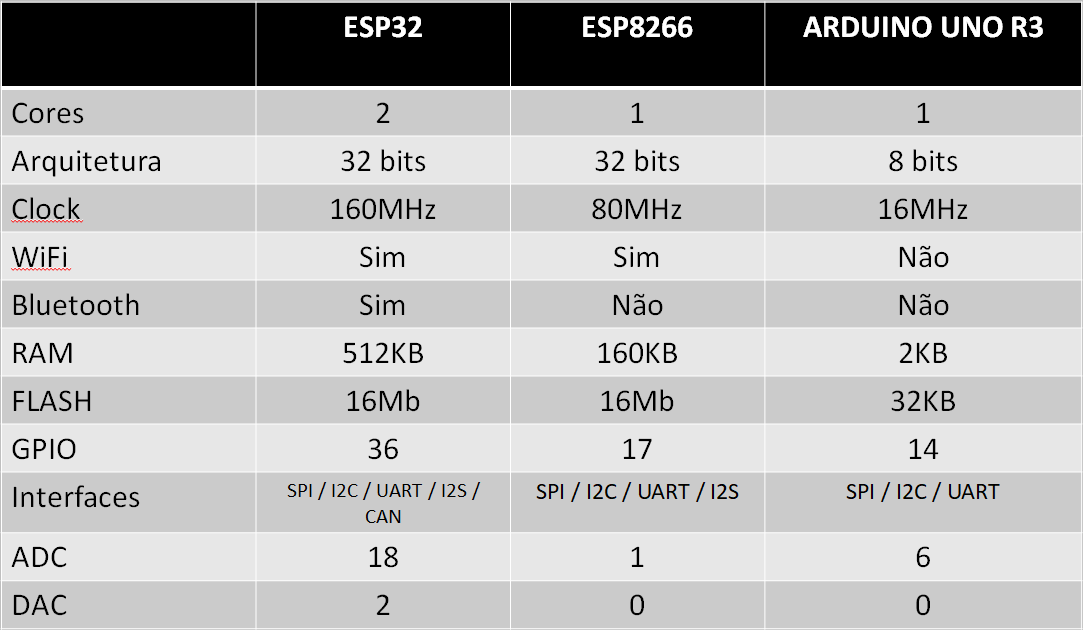
\includegraphics[width=.57\textwidth]{img/esp32-comparation-table.png}
    \caption{Comparativo entre placas de desenvolvimento. Fonte:\cite{esp32-comparation-table}}\label{figTableEsp}
\end{figure}

De acordo com a tabela, o esp32 é \textbf{dual-core}, ou seja, possui dois processadores, tem Wi-Fi e Bluetooth 
integrados e executa programas de 32 bits com memória RAM de 512KB. Portanto, a escolha do esp32 para o desenvolvimento 
do trabalho tem fundamento na robustez do dispositivo em relação aos outros citados, por permitir rodar programas maiores e lidar com mais variáveis simultaneamente (paralelismo), 
essencial para sistemas embarcados que lidam com grandes volumes de dados ou que necessitam de respostas rápidas, sendo esse o caso do sistema em construção. 

\section{Exposição ao monóxido de carbono: riscos e consequências}

O monóxido de carbono (CO) é um gás tóxico, incolor e inodoro, que resulta da combustão incompleta. A intoxicação por esse gás ocorre porque ele se liga preferencialmente à hemoglobina, a proteína 
responsável pelo transporte de oxigênio no sangue, impedindo a distribuição adequada de oxigênio pelo corpo. Como consequência, a hemoglobina se 
torna incapaz de liberar o oxigênio eficientemente nos tecidos, levando a níveis tóxicos de monóxido de carbono no sangue. Isso provoca um aumento na ventilação 
pulmonar na tentativa de compensar a falta de oxigênio, o que agrava os sintomas. O quadro clínico é inespecífico e pode incluir náuseas, aumento da 
frequência respiratória, além de, em casos mais graves, lesões cerebrais e arritmias cardíacas.

Para o diagnóstico, é importante considerar o histórico de exposição a ambientes com potencial risco, como pacientes que estiveram em locais de incêndio. Na medição 
da carboxiemoglobina (COHb) presente no sangue, o paciente pode estar assintomático ou apresentar baixos níveis da substância devido ao curto tempo de exposição, porém somente a medição da taxa de COHb é 
ineficiente para obter informação do nível de lesão causado. No entanto, um eletrocardiograma é um exame eficaz para detectar anormalidades em casos de exposição significativa ao CO. Uma vez detectada 
a intoxicação por monóxido de carbono, o paciente é submetido à terapia com suplementação de oxigênio (O\textsubscript{2}), suporte ventilatório e monitoramento de arritmias cardíacas \cite{carbon-monoxide-poisoning-varon}.

\begin{table}[h!]
    \centering
    \begin{tabular}{|c|c|}
        \hline
        \textbf{COHb \%} & \textbf{Sintomas} \\
        \hline
        10 & Assintomático ou pode ter dor de cabeça \\
        \hline
        20 & Tontura, náusea, dispneia \\
        \hline
        30 & Distúrbios visuais \\
        \hline
        40 & Confusão, síncope \\
        \hline
        50 & Convulsões e coma \\
        \hline
        >= 60 & Disfunção cardiopulmonar e morte \\
        \hline
    \end{tabular}
    \caption{Sintomas de Envenenamento Agudo por CO baseados nos níveis de COHb. Fonte: Retirado e traduzido de \cite{carbon-monoxide-poisoning-varon}}
\end{table}

\section{Trabalhos relacionados}

O desenvolvimento de trabalhos na área de IoT focados em monitoramento de condições ambientes e prevenção de acidentes 
possuem uma vasta literatura disponível, evidenciando o potencial de atuação dos sistemas embarcados e distribuídos para 
o uso nos mais diversos setores, como indústrias, hospitais e residências. Portanto, nesse conteúdo  serão discutidas 
algumas das soluções que serviram como base para o presente trabalho. 

O trabalho \textit{Sumaúma: estação de monitoramento de plantas domésticas utilizando android e esp32} \cite{ufam-aosp-sumama} é a proposta de 
referência deste trabalho de conclusão de curso, onde o autor descreve uma solução utilizando o AOSP para a construção de um 
sistema embarcado de monitoramento da estação de planta. Os dispositivos utilizados foram o microcontrolador esp32 NodeMCU e os sensores DHT11 (temperatura e umidade do ar), LDR 
(luminosidade) e FC-28 (umidade do solo), pois o protótipo realiza a medição em tempo real e exibe os dados coletados na interface gráfica do aplicativo Android. 

Na proposta apresentada, o objetivo da customização do Android foi atender demandas específicas do projeto e comunicar os dados na camada de usuário, resultando na criação de um novo produto com base no 
circuito eletrônico da estação de monitoramento.  As modificações realizadas incluem o desenvolvimento do \textit{firmware} na ESP, 
da HAL (\textit{Hardware Abstration Layer}), do \textit{Manager}, do \textit{Driver} e da biblioteca. O resultado final foi uma estação inteligente de monitoramento 
de planta, combinando hardware e software dentro da plataforma Android, porém, para trabalhos futuros, o autor propõe como melhoria a integração do sistema 
com outros de automação residencial, pois o protótipo não possui conexão de internet e funciona com dependência de conexão física 
entre o microcontrolador e o \textit{smartphone}.

\begin{figure}[ht]
    \centering
    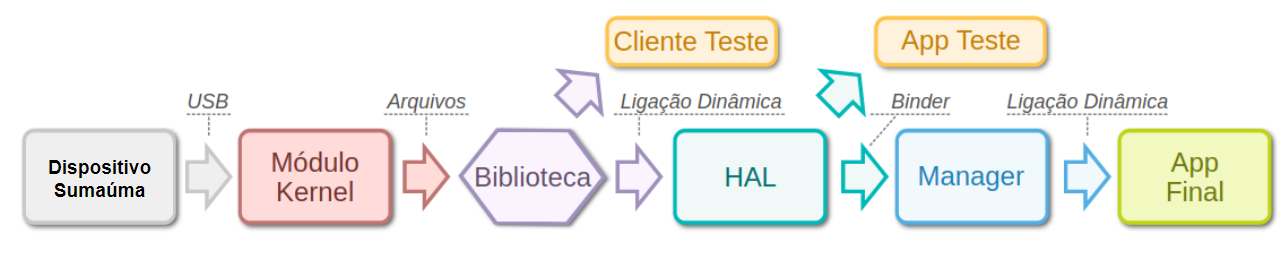
\includegraphics[width=.87\textwidth]{img/smartlamp-overview.png}
    \caption{Personalização do Android. Fonte:\cite{ufam-aosp-sumama}}\label{figSumauma}
\end{figure}

O projeto de Sá, por sua vez, focou no uso de dispositivos na área de IoT para a prevenção de incêncios em ambientes residenciais \cite{uea-iot-deteccao-incendio}. O trabalho 
foca em uma solução web para monitoramento de variáveis com uso do módulo NodeMCU ESP12, pois o microcontrolador envia dados de temperatura, gás inflamável e de 
fumaça por rede Wi-Fi para o backend da aplicação, feito em MySQL e PHP. No componente de hardware, os sensores utilizados foram o BM280 (Sensor de temperatura digital) e MQ2 (Sensor de gás/fumaça), assim como 
o atuador do tipo válvula para acionar o desligamento de gás de cozinha em situação de vazamento, evitando incêndio ou minimizando seus efeitos. 

Além disso, foi utilizada uma bateria de lítio recarregável para garantir a autonomia do dispositivo, tornando o sistema mais independente. Para a proteção e acomodação dos componentes eletrônicos, foi 
confeccionado um \textit{case} personalizado por meio de impressão 3D, o que conferiu acabamento e proteção ao protótipo. A autora também desenvolveu uma placa de circuito impresso (PCB), na qual integrou os sensores, atuadores e
a conexão com o microcontrolador.

Para validar o protótipo, realizaram-se diversos tipos de testes e simulações, incluindo a simulação de fumaça, em que o dispositivo foi colocado em uma caixa com 
fumaça confinada, além de testes com variação de temperatura e queima de papel para detecção de incêndio e emissão de alerta sonoro. Portanto, o sistema é eficaz às mudanças do ambiente e 
tem a vantagem de exibir os dados em tempo real, garantindo uma resposta ágil em situações de perigo. 

\begin{figure}[ht]
    \centering
    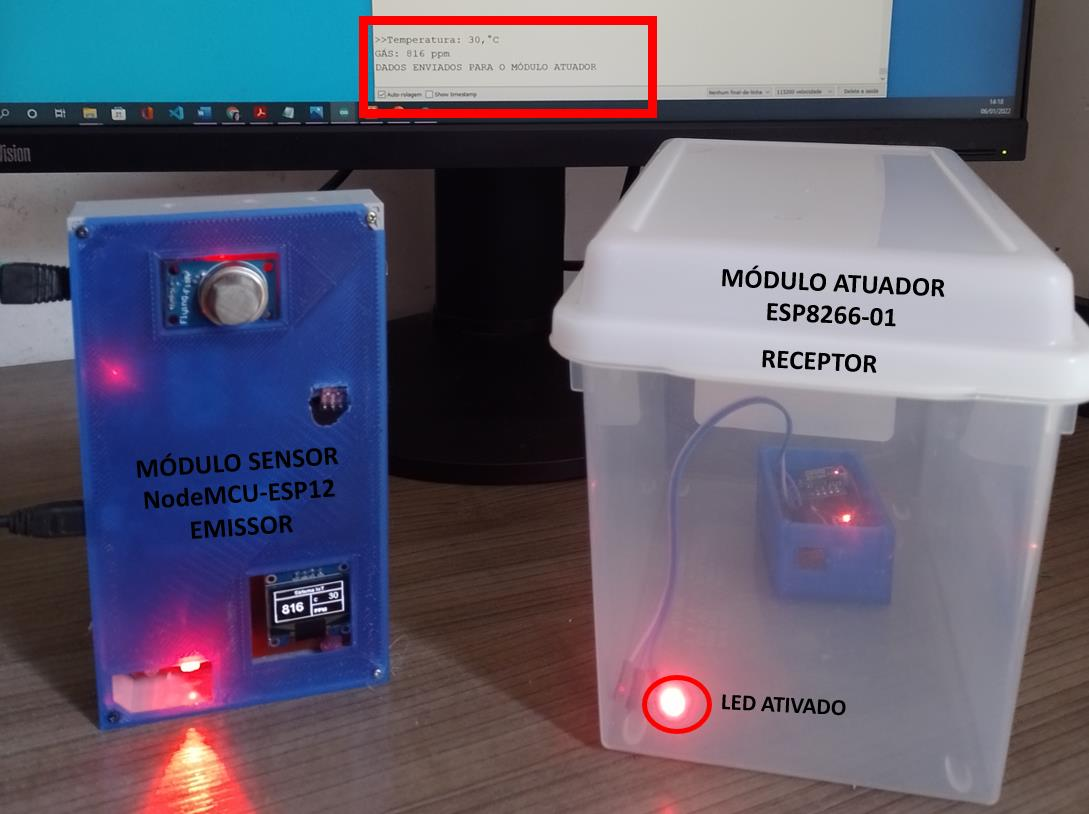
\includegraphics[width=.44\textwidth]{img/sa-dispositivo-simulacao.png}
    \caption{Dispositivo em situação de fumaça. Fonte:\cite{uea-iot-deteccao-incendio}}\label{figProtitpoUEA}
\end{figure}

Em \textit{Indoor Air Quality Monitoring on AWS Using MQTT Protocol} \cite{iot-monitoring-on-aws}, os autores mostram o desenvolvimento de 
um módulo de monitoramento da qualidade do ar em ambientes internos utilizando o protocolo MQTT e serviços da AWS. O módulo 
proposto utiliza sensores para medir a qualidade do ar interno, incluindo CO\textsubscript{2}, O\textsubscript{2} e poeira, com os dados sendo enviados e armazenados na 
nuvem para uma visualização em tempo real. O sistema alerta o usuário caso a qualidade do ar seja inadequada. 

O trabalho entitulado ``SISTEMA DE DETECÇÃO DE GÁS PARA ÁREAS DE RISCOS (SDGRL)'' sugere um  sistema que identifica vazamentos de gás em ambientes 
domésticos e que avisa sobre a situação aos responsáveis, além disso, toma as primeiras ações para reduzir inerentes ao fato, para isso utiliza um sensor 
MQ-5 integrado a um microcontrolador Arduino, também utiliza um módulo relé e uma válvula solenóide, também utiliza o SHIELD GSM ARDUINO 2 para comunicação com o usuário \cite{sistema-deteccao}. 

O projeto ``Automação residencial de monitoramento de gás por meio da plataforma Arduino e IOT'' teve como objetivo descrever a implementação de um sistema de automação residencial 
inteligente para monitoramento e alerta de vazamento de gás utilizando a Internet das Coisas (IoT), o sistema consiste em um microcontrolador Arduino UNO conectado a um sensor de gás MQ-5 e um 
módulo bluetooth HC-05, que envia os dados para um aplicativo Android desenvolvido na plataforma Android Studio. O aplicativo exibe em tempo real o nível de gás detectado e emite alerta visuais e 
sonoros quando a concentração ultrapassa uma certa porcentagem, além de armazenar os registros de vazamento em um servidor \cite{alexandre-automaccao-formulas-de-leitura-sensor}.